\documentclass{beamer}

\usetheme{Warsaw}

\usepackage{ctex}

\usepackage{mathrsfs}

\usepackage{amsmath, amsthm, amssymb}

\title{花巷:一个用于进行非共价相互作用指数(NCI)分析的脚本}

\author[qidawei98@outlook.com]{王秀 \inst{1}\inst{2}  \and 戚达炜 \inst{1}\inst{2}}

\institute{\inst{1} 物理与能源学院,福建师范大学 \and  \inst{2} 福建物质结构研究所,中国科学院}

\date{}

\begin{document}

\begin{frame}
\titlepage
\end{frame}

\begin{frame}{理论}
%非共价相互作用指数(NCI)理论由量子化学家Erin Johnson在杨伟涛课题组读博时提出。

Johnson, E. R., Keinan, S., Mori-Sánchez, P., Contreras-García, J., Cohen, A. J. \& Yang, W. (2010). J Am Chem Soc 132, 6498–6506.
\begin{definition}
\[
\text{RDG} = \frac{|\nabla \rho(\mathbf{r})|}{2(3\pi^2)^{1/3} \rho(\mathbf{r})^{4/3}}
\]
\end{definition}
在$\text{RDG}=0.5 a.u.$的位置画等值面。
$
H(\rho) = \begin{pmatrix}
\frac{\partial^2 \rho}{\partial x^2} & \frac{\partial^2 \rho}{\partial x \partial y} & \frac{\partial^2 \rho}{\partial x \partial z} \\
\frac{\partial^2 \rho}{\partial y \partial x} & \frac{\partial^2 \rho}{\partial y^2} & \frac{\partial^2 \rho}{\partial y \partial z} \\
\frac{\partial^2 \rho}{\partial z \partial x} & \frac{\partial^2 \rho}{\partial z \partial y} & \frac{\partial^2 \rho}{\partial z^2}
\end{pmatrix}
$三个特征值$\lambda_1, \lambda_2$, and $\lambda_3$

等值面的颜色由$\rho\operatorname{sign}(\lambda_2)$给出,越偏向于负值(冷色)相互作用约偏向于吸引,越偏向于正值(暖色)相互作用约偏向于排斥。
\end{frame}

\begin{frame}{算法}
求解的重点在于各种类型的数值导数。

常规算法往往结合了插值和快速傅里叶变换,在倒空间求解。

我们的程序充分利用计算机的性能,在实空间中进行有限差分:
\begin{align}
f(x_0 + h) &= f(x_0) + hf'(x_0) + \frac{h^2}{2!}f''(x_0) + \mathcal{O}(h^3) \\
f(x_0 - h) &= f(x_0) - hf'(x_0) + \frac{h^2}{2!}f''(x_0) + \mathcal{O}(h^3)
\end{align}
$$
\Longrightarrow f'(x_0) = \frac{f(x_0 + h) - f(x_0 - h)}{2h}
$$
计算所需的数据点由径向基函数查询得到。根据具体的任务和CPU的类型分配并行计算。

我们算法的结果与理想情况下的数值解更加接近。
\end{frame}

\begin{frame}{示例 mp-1218409 SrCaAl2(SiN3)2}
    \begin{columns}[T] % The [T] option aligns the columns at the top
        \begin{column}{0.5\textwidth}
            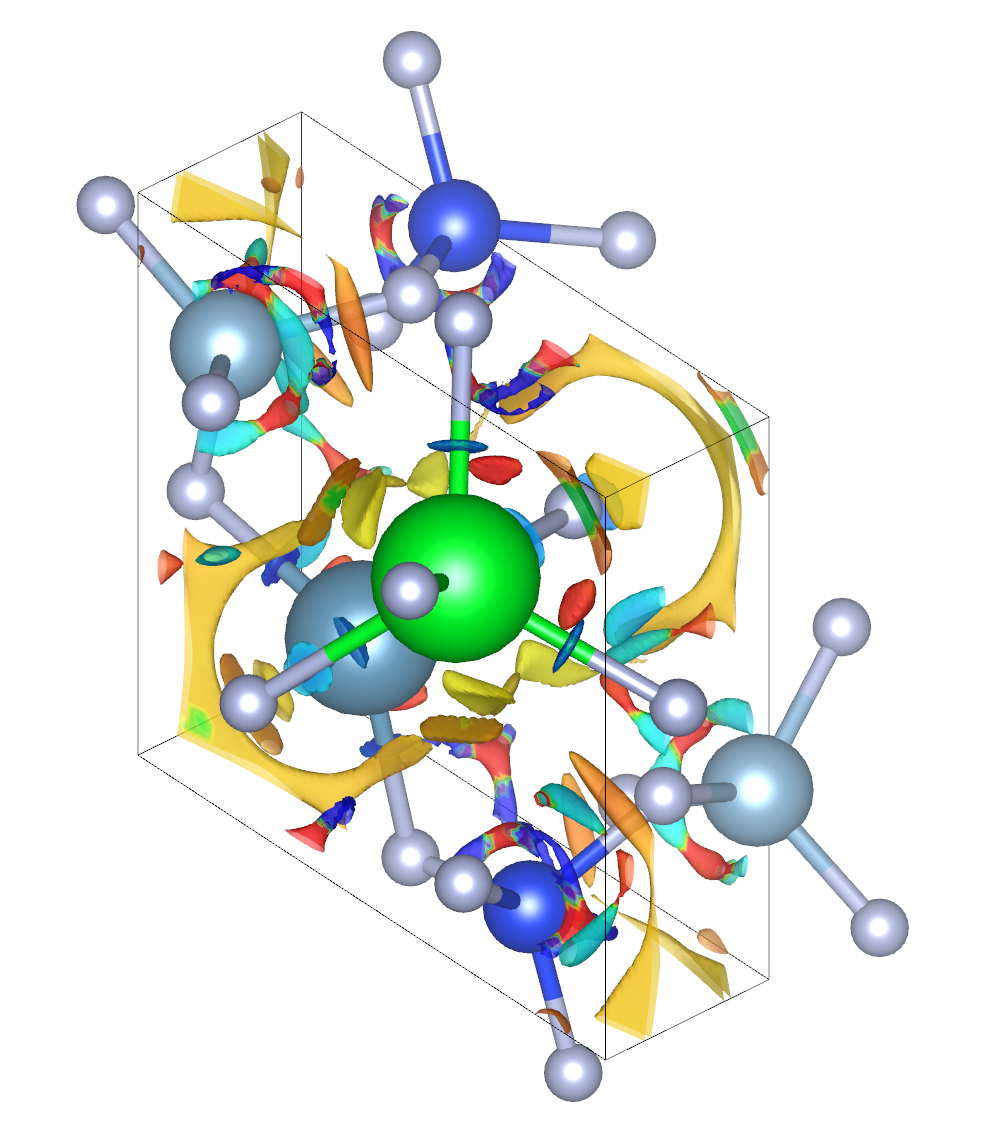
\includegraphics[scale=0.3]{1}
        \end{column}
        \begin{column}{0.5\textwidth}
            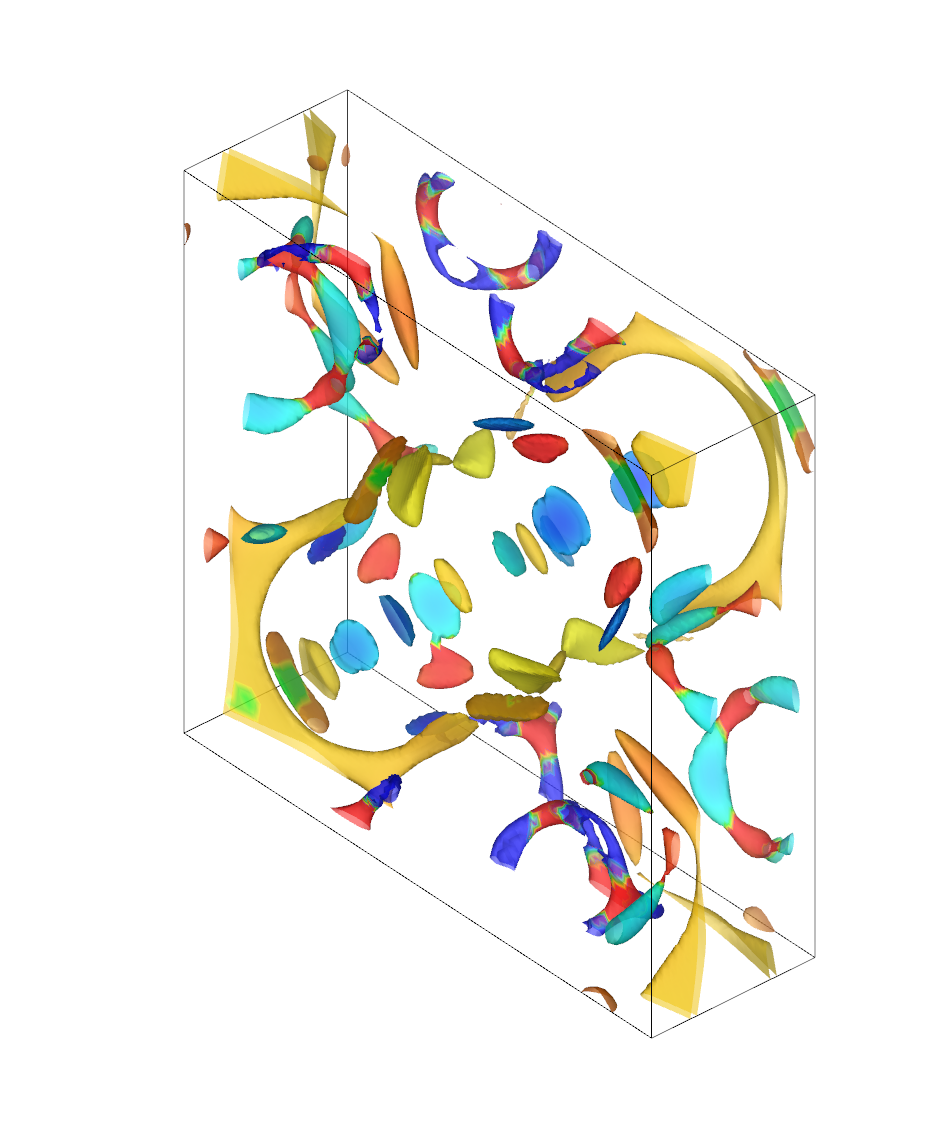
\includegraphics[scale=0.3]{2}
        \end{column}
    \end{columns}
\end{frame}
\end{document}